\documentclass[a4paper]{scrartcl}
\usepackage{amsmath,amssymb,amsthm}
\usepackage{bm}
\usepackage{biblatex}
\usepackage{caption}
\usepackage{float}
\usepackage[colorlinks=true, allcolors=black, urlcolor=cyan]{hyperref}
\usepackage{graphicx}
\usepackage[framed,numbered]{matlab-prettifier}
\usepackage{mathtools}
\usepackage{mcode}
\usepackage{physics}
\usepackage{siunitx}
\usepackage{cancel}
\usepackage{appendix}

\renewcommand{\thesection}{\Roman{section}}
\renewcommand{\thesubsection}{\roman{subsection})}

\title{Assignment 4}
\subtitle{ELEC 442 - Introduction to Robotics}
\author{Sondre Myrberg (81113433) \and Ola Helbaek (68776772)}


\setlength{\parindent}{0pt} % Disable indentation
\mathtoolsset{showonlyrefs} % Only show equation numbers on referenced equations

\def\undertilde#1{\mathord{\vtop{\ialign{##\crcr
$\hfil\displaystyle{#1}\hfil$\crcr\noalign{\kern1.5pt\nointerlineskip}
$\hfil\widetilde{}\hfil$\crcr\noalign{\kern1.5pt}}}}} %Lousy way, but need this undertilde
\newcommand{\me}[1]{\mathrm{e}^{#1}}


\begin{document}

\hypersetup{pageanchor=false}
\begin{titlepage}
    \maketitle
    \vfill
    \vfill
    \vfill
    \vfill
    
\includegraphics[width=0.95\textwidth]{../../ubc_logo.pdf}
    \vfill
    \vfill
\end{titlepage}
\hypersetup{pageanchor=true}

\section{Two-Link Manipulator Open Loop Simulation}
Considering the two link manipulator described on page 87 in chapter 6 of the notes, the equations of motion are given by equation (209) to (233). In general we have the Euler-Lagrange equations of motion given as
\begin{equation}
	\begin{aligned}
		\dv{t}\left[\pdv{L}{\dot{q}_i} (q,\dot{q}) \right] - \pdv{L}{q_i} (q,\dot{q}) &= \tau_i \\
	\end{aligned}
\end{equation}
where
\begin{equation}
	\begin{aligned}
		L(\bm{q},\dot{\bm{q}}) &= T(\bm{q},\dot{\bm{q}}) - V(\bm{q})
	\end{aligned}
\end{equation}
and $\tau_i$ is the generalized force or torque associated with coordinate $i$. This can be written on standard form as
\begin{equation}
	\begin{aligned}
		D(\bm{q})\ddot{\bm{q}} + C(\bm{q},\dot{\bm{q}})\dot{\bm{q}} + G(\bm{q}) &= \bm{u} + \underline{J}^\top_n \begin{bmatrix} \underline{f}_e \\ \underline{\tau}_e \end{bmatrix}
	\end{aligned}
\end{equation} 
where the last term can be ignored as we do not interact with the environment. This gives us the secod order system
\begin{equation}
	\begin{aligned}
		\ddot{\bm{q}} &= D^{-1}(\bm{q})\left[\bm{u} - C(\bm{q},\dot{\bm{q}})\dot{\bm{q}} - G(\bm{q}) \right]
	\end{aligned}
\end{equation}
with $D(\bm{q})$ given by equation (222), $C(\bm{q},\dot{\bm{q}})$ given by (232) and $G(\bm{q})$ by (233), and $\bm{q} = \begin{bmatrix}
	\theta_1 \\ \theta_2
\end{bmatrix}$. To generate these matrices in Simulink, we implement block functions shown in \autoref{fig:genC}, \autoref{fig:genD} and \autoref{fig:genG} in \autoref{sec:simulink}. The complete mainpulator dynamics are implemented in \autoref{fig:dynamics}.

\subsection{}
With $\bm{x}(0) = \begin{bmatrix}0 & 0 & 0 & 0\end{bmatrix}^\top$ and $\tau_1 = \tau_2 = 0$ we get the response shown in \autoref{fig:1i_1}.

\begin{figure}[ht!]
	\centering
	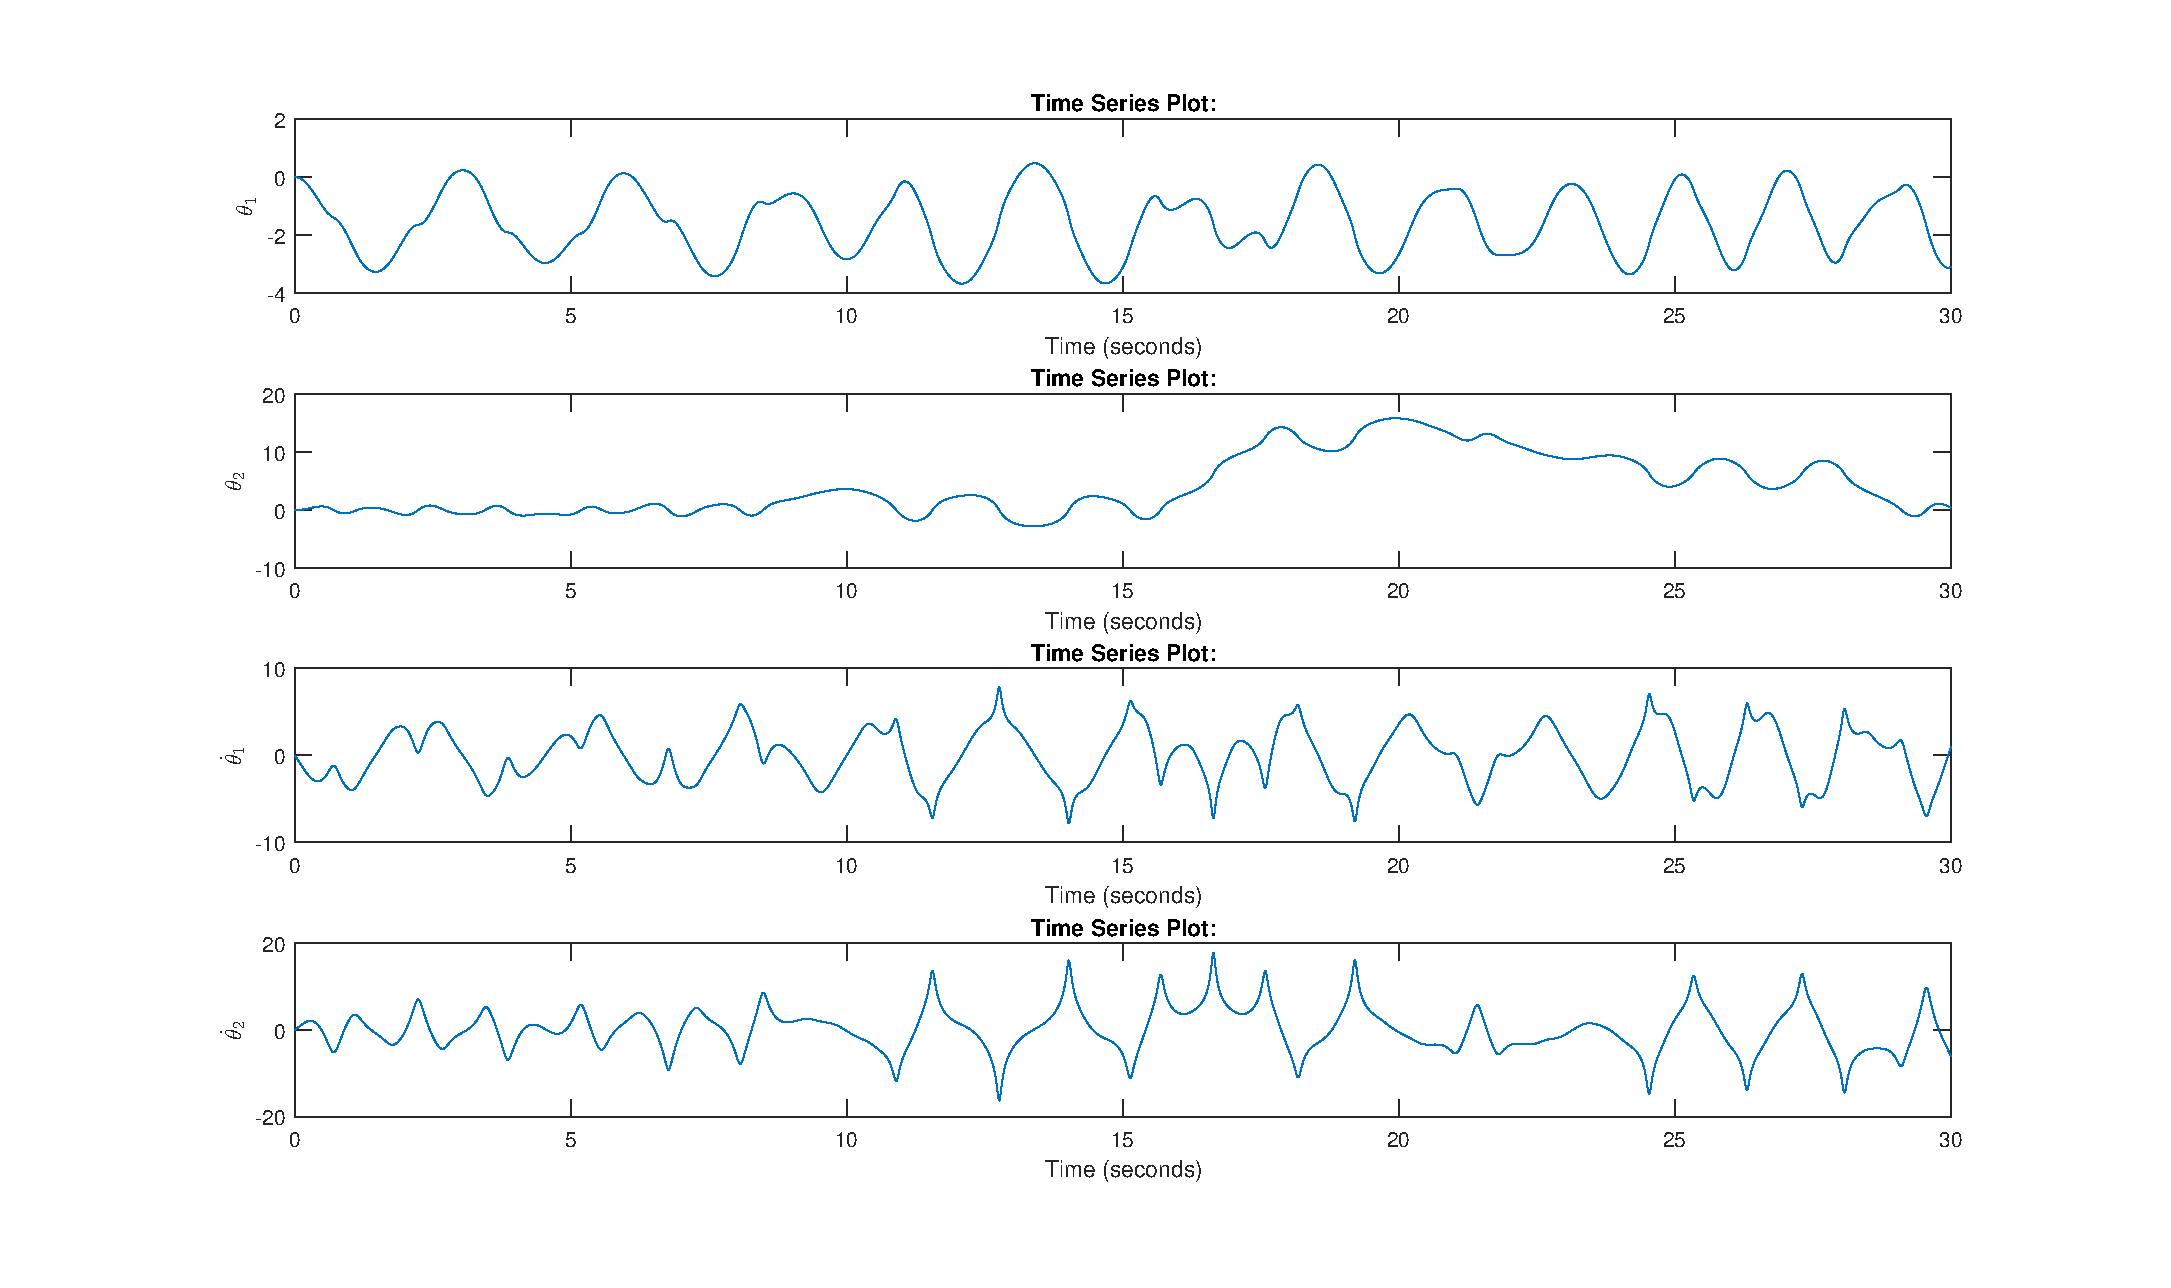
\includegraphics[width=.90\textwidth]{fig/1i_1.eps}
	\caption{Response of all states with all states initialized to zero}
	\label{fig:1i_1}
\end{figure}

\subsection{}
With $\bm{x}(0) = \begin{bmatrix}0 & \tfrac{\pi}{2} & 0 & 0\end{bmatrix}^\top$ and $\tau_2 = \SI{5}{Nm}$ we get the response shown in \autoref{fig:1ii_1}. Here the total energy of the system is increasing, which is seen in the plots for the angular velocities.

\begin{figure}[ht!]
	\centering
	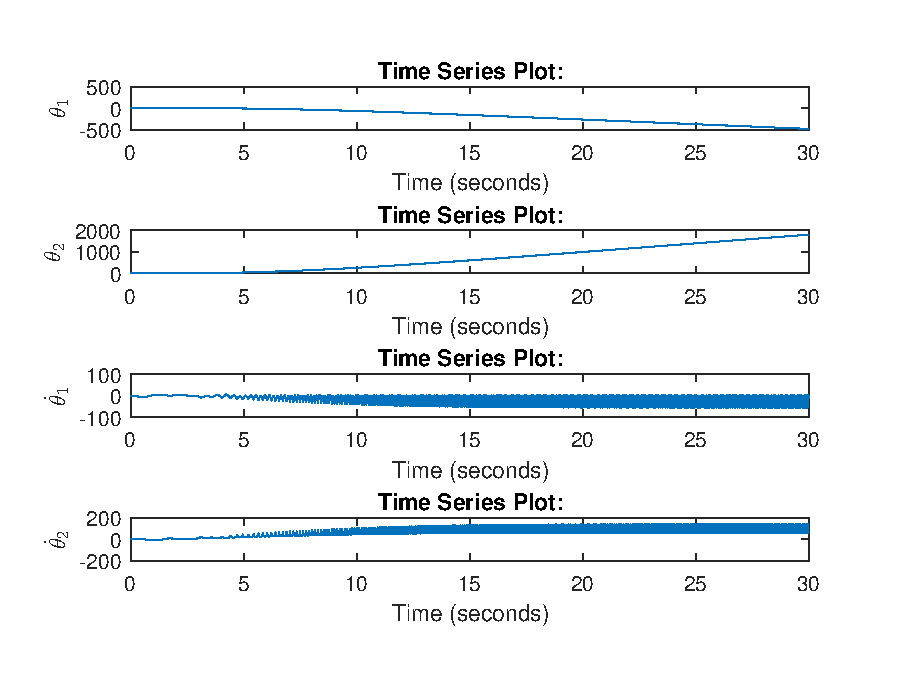
\includegraphics[width=.90\textwidth]{fig/1ii_1.eps}
	\caption{Response of all states with  $\bm{x}(0) = \left[0 \: \tfrac{\pi}{2} \: 0 \: 0\right]^\top$ and $\tau_2 = \SI{5}{Nm}$}
	\label{fig:1ii_1}
\end{figure}

\subsection{}
With $\bm{x}(0) = \begin{bmatrix}0 & 0 & 0 & 0\end{bmatrix}^\top$ and friction modeled as $\tau_1 = -0.5\dot{\theta}_1$ and $\tau_2 = -0.5\dot{\theta}_2$ we get the response shown in \autoref{fig:1iii_1}. Here we see that the amplitude is decreasing, wich makes sense because the total energy of the system is decreasing when friction is added.

\begin{figure}[ht!]
	\centering
	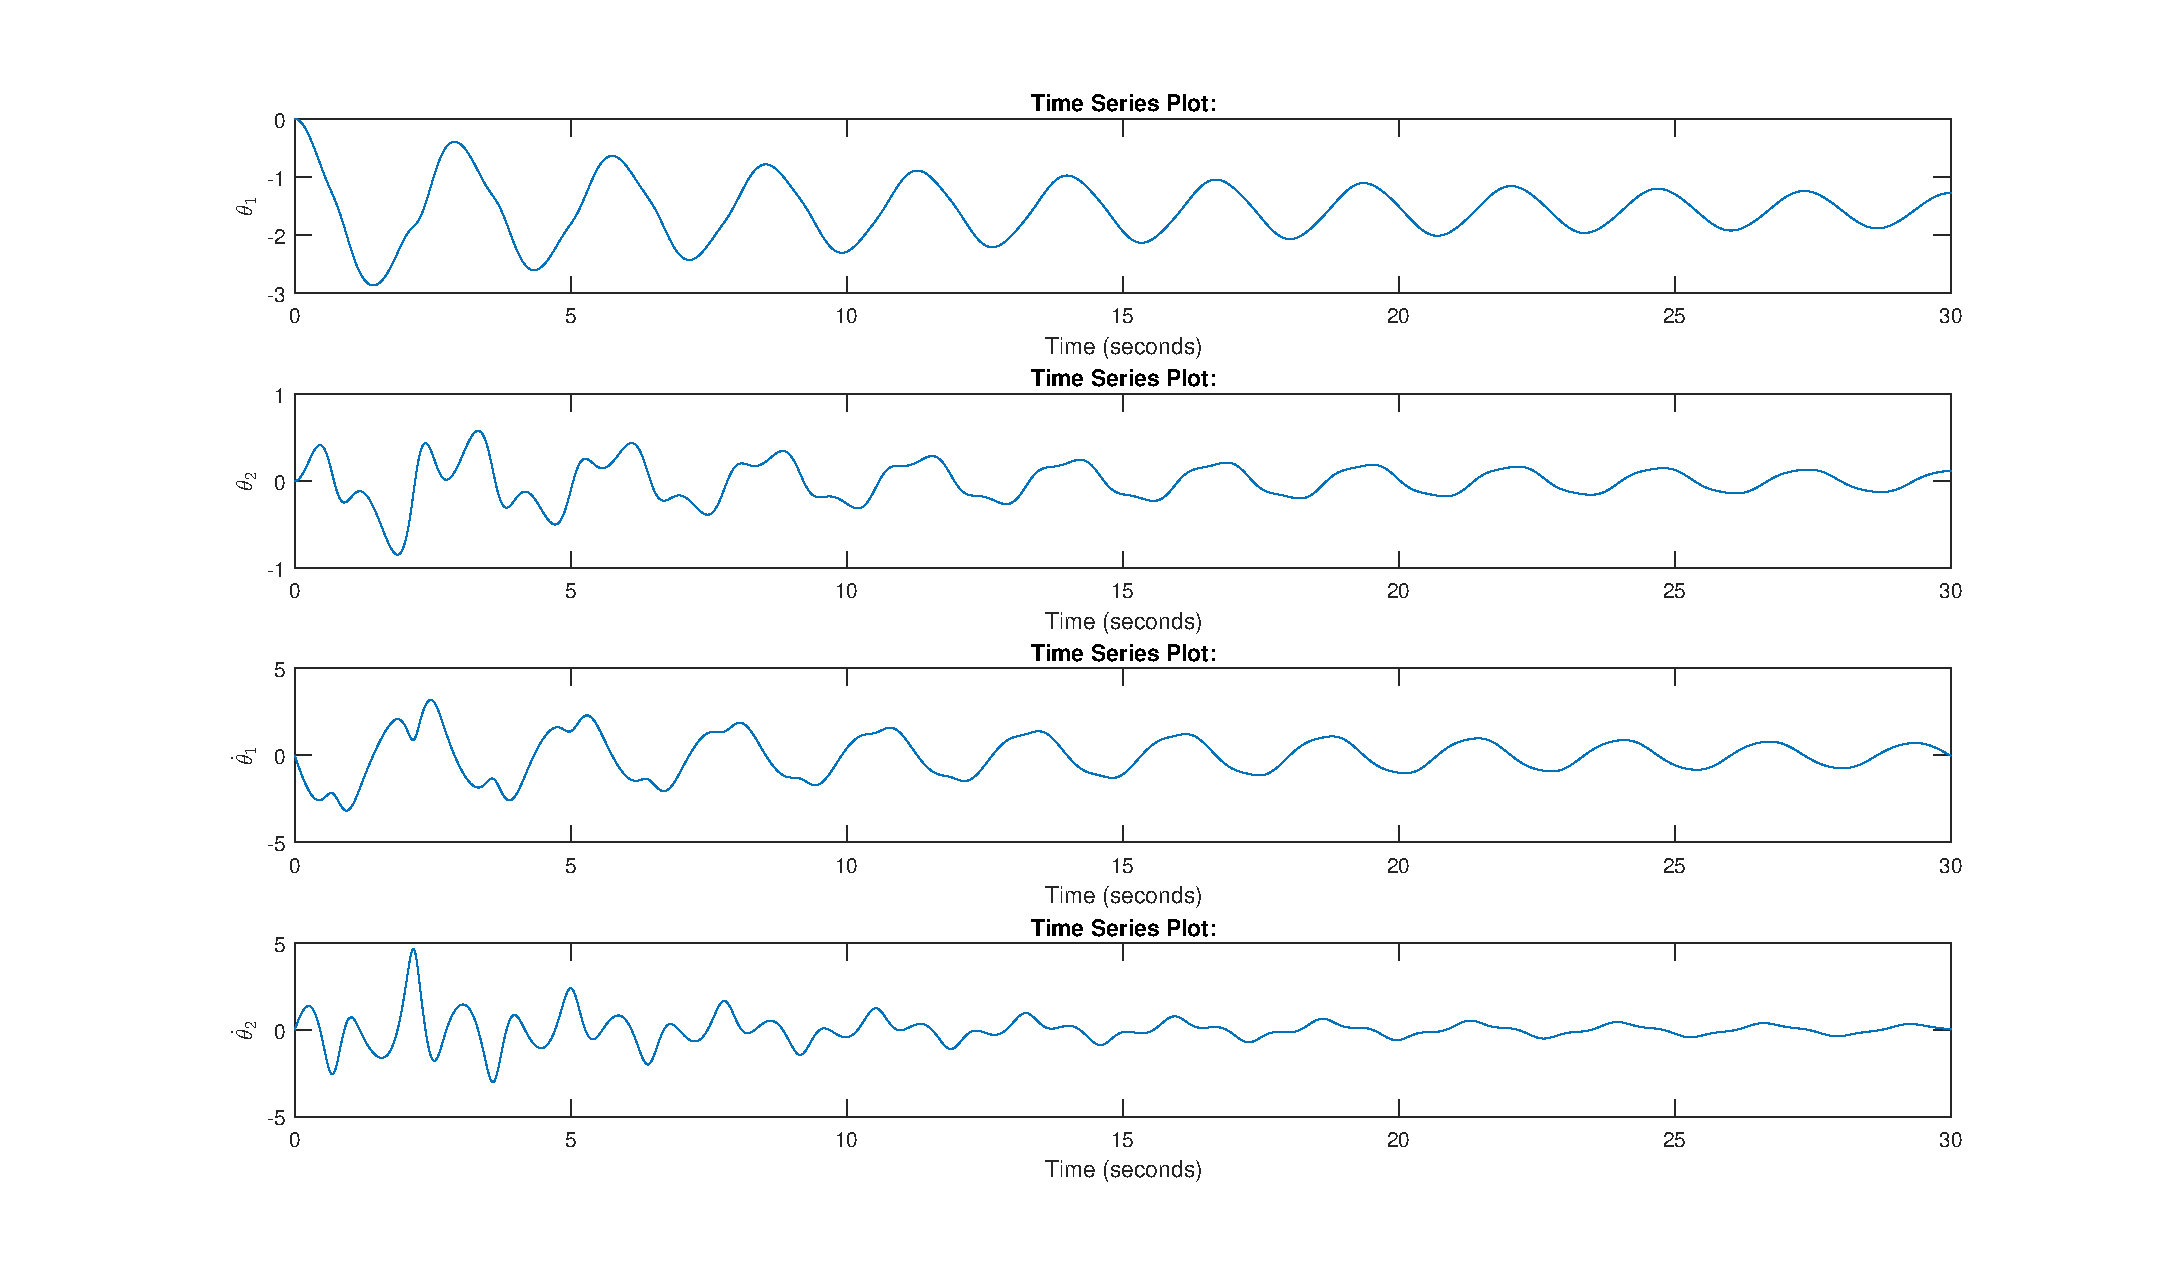
\includegraphics[width=.90\textwidth]{fig/1iii_1.eps}
	\caption{Response of all states with  all states initialized to zero and friction modeled as  $\tau_1 = -0.5\dot{\theta}_1$ and $\tau_2 = -0.5\dot{\theta}_2$ }
	\label{fig:1iii_1}
\end{figure}

\section{Controller Implementation}\label{sec:controller}
\subsection{Closed loop joint-space control}
With the PD + gravity set point controller we get the input vector
\begin{equation}
	\begin{aligned}
		\bm{u} &= \underbrace{G(\bm{q})}_{\text{Gravity terms}} + \underbrace{K_p(\bm{q}_d - \bm{q}) - K_v (\dot{\bm{q}}_d - \dot{\bm{q}})}_{\text{PD-controller}}
	\end{aligned}
\end{equation}
where we require
\begin{equation}
	K_p, K_v \succ 0
\end{equation}
which is implemented as the Simulink diagram shown in \autoref{fig:PDgravity}. With this implementation and the initial conditions 
\begin{equation}
	\begin{aligned}
		\bm{x}(0) &= \begin{bmatrix} -\tfrac{\pi}{2} & 0 & 0 & 0 \end{bmatrix}^\top \\
		\bm{q}_d &= \begin{bmatrix} 0 & \tfrac{\pi}{2} \end{bmatrix}^\top \\
		\dot{\bm{q}}_d &= \begin{bmatrix} 0 & 0 \end{bmatrix}^\top \\
		K_p &= \begin{bmatrix} 1 & 0 \\ 0 & 1 \end{bmatrix}\\
		K_v &= \begin{bmatrix} 2 & 0 \\ 0 & 2 \end{bmatrix}\\
	\end{aligned}
\end{equation}
we get the output shown in \autoref{fig:2PD_1}.

\begin{figure}[ht]
	\centering
	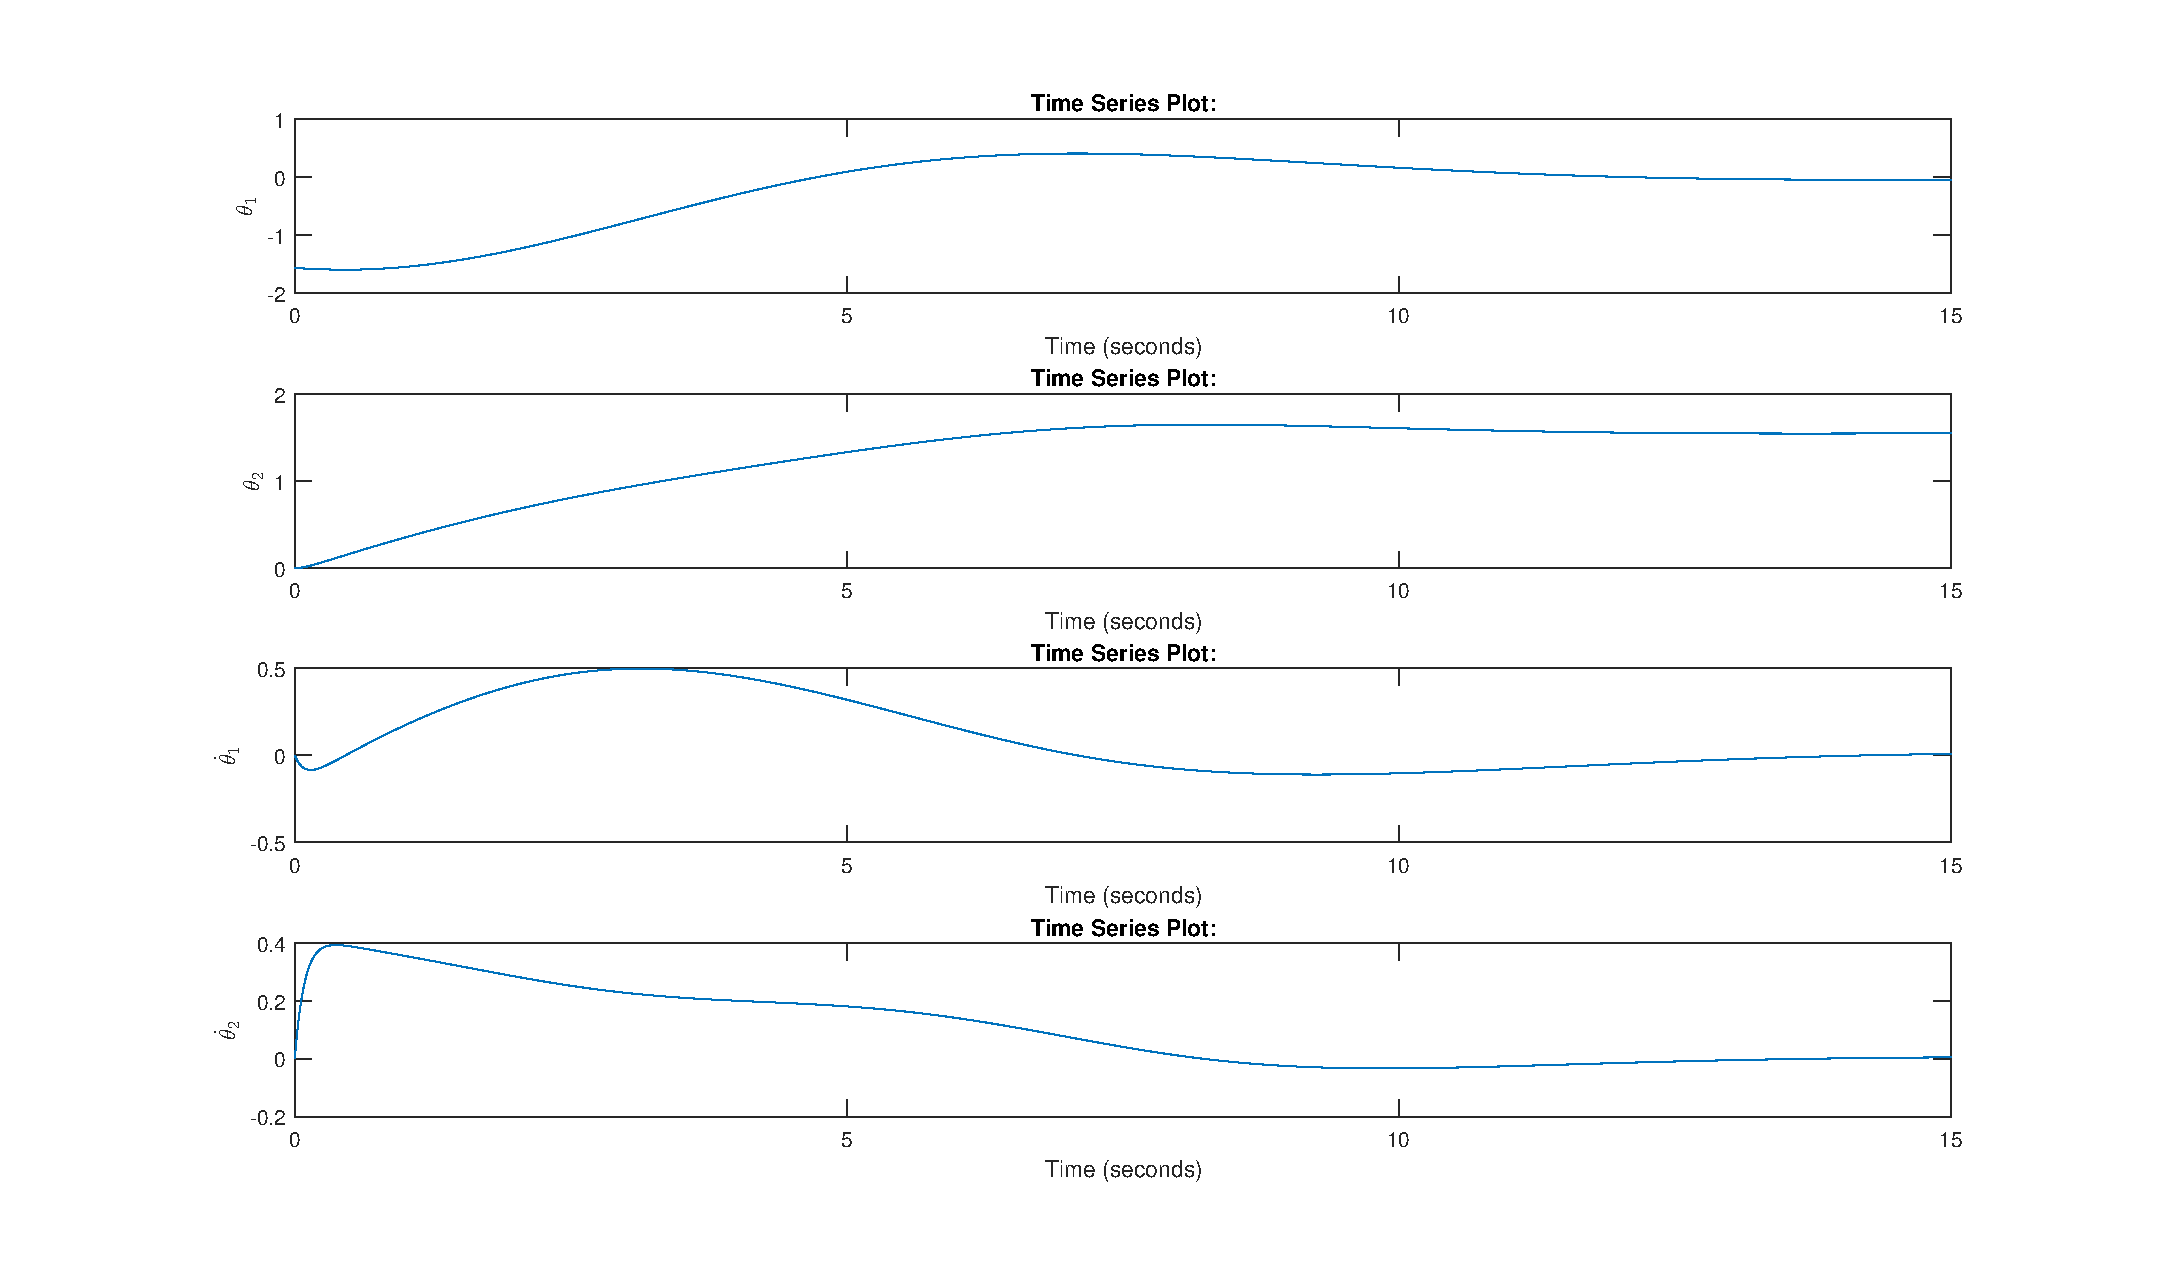
\includegraphics[width=0.95\textwidth]{fig/2PDg_1.eps}
	\caption{Output states with the PD + gravity controller}
	\label{fig:2PD_1}
\end{figure}

\subsection{Closed loop Cartesian-space control}\label{ssec:stiffness}
When we consider the 2DOF double pendulum there are a lot fo terms we can ignore as they will cancel out anyway. The orientation error and angular velocities are not to be considered, and also the position along the $\bm{k}$-axis can be ignored. This results in the control law
\begin{equation}
	\begin{aligned}
		\bm{u} &= G(\bm{q}) + J^\top \begin{bmatrix} \underline{\bm{f}}_n \\ \underline{\bm{\tau}}_n \end{bmatrix}\\
		 \begin{bmatrix} \underline{\bm{f}}_n \\ \underline{\bm{\tau}}_n \end{bmatrix} &= K_p(\bm{o}_d - \bm{o}_n) + K_v(\dot{\bm{o}}_d - \dot{\bm{o}}_n) 
	\end{aligned}
\end{equation}
where $J$ is given by the $\bm{i}$- and $\bm{j}$-components of
\begin{equation}
	\begin{bmatrix}
		\bm{k}_0 \cross (\bm{o}_n - \bm{o}_0) & \bm{k}_1 \cross (\bm{o}_n - \bm{o}_1) \\
		\bm{k}_0 & \bm{k}_1
	\end{bmatrix}
\end{equation}
and
\begin{equation}
\begin{aligned}
	\bm{o}_0 &= \bm{0}^\top \\
	\bm{o}_n &= \bm{o}_2\\
	\bm{o}_1 - \bm{o}_0 &= \begin{bmatrix} l_1 \cos\theta_1 \\ l_1 \sin\theta_1 \\ 0 \end{bmatrix}\\
	\bm{o}_2 - \bm{o}_0 &= \begin{bmatrix} l_1 \cos\theta_1 + l_2 \cos(\theta_1 + \theta_2)\\
	l_1 \sin\theta_1 + l_2 \sin(\theta_1+\theta_2) \\ 0 \end{bmatrix}\\
	\bm{o}_2 - \bm{o}_1 &= \begin{bmatrix}l_2 \cos(\theta_1 + \theta_2) \\ l_2 \sin(\theta_1 + \theta_2) \\ 0\end{bmatrix}
\end{aligned}
\end{equation}
This gives
\begin{equation}
	\begin{aligned}
		\dot{\bm{o}}_n &= \begin{bmatrix}
			-l_1 \sin\theta_1\dot{\theta}_1 - l_2\sin(\theta_1 + \theta_2)(\dot{\theta}_1 + \dot{\theta}_2) \\
			l_1 \cos\theta_1\dot{\theta}_1 + l_2\cos(\theta_1 + \theta_2)(\dot{\theta}_1 + \dot{\theta}_2) \\
			0
		\end{bmatrix}
	\end{aligned}
\end{equation}
and
\begin{equation}
	J = \begin{bmatrix}
			-l_1\sin\theta_1 - l_2\sin(\theta_1 + \theta_2) & - l_2\sin(\theta_1 + \theta_2)\\
			l_1\cos\theta_1 + l_2\cos(\theta_1 + \theta_2) & l_2\cos(\theta_1 + \theta_2)\\
			0 & 0\\
			\bm{k} & \bm{k}
		\end{bmatrix}
\end{equation}
Again, we have a 2DOF manipulator, so we only have use the first two elements of our vectors, giving us
\begin{equation}
	\begin{aligned}
		\bm{u} = G(\bm{q}) + J^\top \Bigg[ &K_p\left(\bm{o}_d - \begin{bmatrix}l_1 \cos\theta_1 + l_2 \cos(\theta_1 + \theta_2)\\l_1 \sin\theta_1 + l_2 \sin(\theta_1+\theta_2) \end{bmatrix}\right) \\
		+ &K_v\left(\dot{\bm{o}}_d - \begin{bmatrix} -l_1 \sin\theta_1\dot{\theta}_1 - l_2\sin(\theta_1 + \theta_2)(\dot{\theta}_1 + \dot{\theta}_2) \\
			l_1 \cos\theta_1\dot{\theta}_1 + l_2\cos(\theta_1 + \theta_2)(\dot{\theta}_1 + \dot{\theta}_2)\end{bmatrix} \right) \Bigg]\\
		J = &\begin{bmatrix}
			-l_1\sin\theta_1 - l_2\sin(\theta_1 + \theta_2) & - l_2\sin(\theta_1 + \theta_2)\\
			l_1\cos\theta_1 + l_2\cos(\theta_1 + \theta_2) & l_2\cos(\theta_1 + \theta_2)
		\end{bmatrix}
	\end{aligned}
\end{equation}
The simulink diagram to generate the Jacobian is shown in \autoref{fig:genJ} and the simulink diagram for the stiffness controller is shown in \autoref{fig:stiffness}. To change between the different $K_p$'s simply comment and uncomment in the MATLAB file as seen in \autoref{sec:matlab},  as all constants are defined there. When changing controller, simply connect the deired controller in the simulink file shown in \autoref{fig:system} and run the associated script. With $K_p = \text{diag}(1,1)$ we get the response shown in \autoref{fig:2stiff1_1}, with $K_p = \text{diag}(0.2,1)$ the response is shown in \autoref{fig:2stiff02_1} and with $K_p = \text{diag}(1,0.2)$ it's shown in \autoref{fig:2stiff1_02}. From this we see that even though we have the same initial position and desired end effector location we get fundamentally different trajectories. 

\begin{figure}[ht]
	\centering
	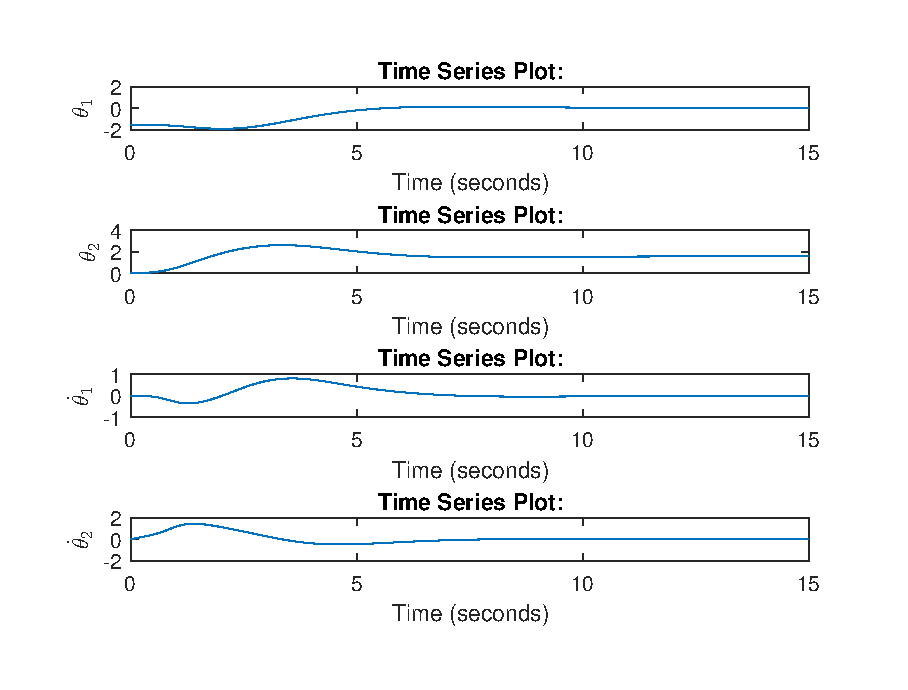
\includegraphics[width=0.75\textwidth]{fig/2stiff_11.eps}
	\caption{Response of the double pendulum with $K_p = \text{diag}(1,1)$}
	\label{fig:2stiff1_1}
\end{figure}
\begin{figure}[ht]
	\centering
	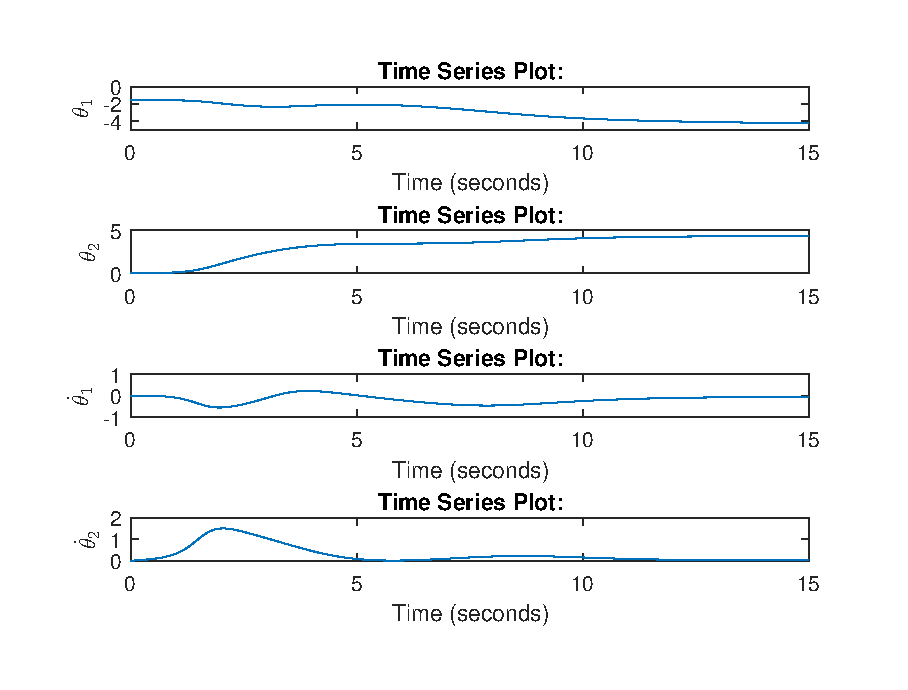
\includegraphics[width=0.75\textwidth]{fig/2stiff_021}
	\caption{Response of the pwndulum with $K_p = \text{diag}(0.2,1)$}
	\label{fig:2stiff02_1}
\end{figure}
\begin{figure}[ht]
	\centering
	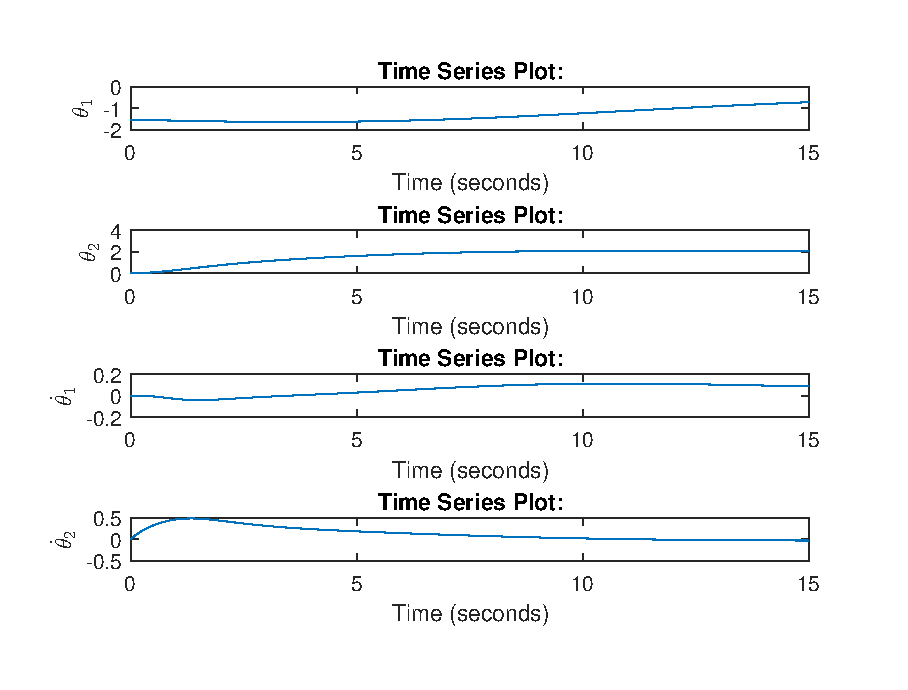
\includegraphics[width=0.75\textwidth]{fig/2stiff_102}
	\caption{Response of the pwndulum with $K_p = \text{diag}(1,0.2)$}
	\label{fig:2stiff1_02}
\end{figure}


\clearpage
\appendix
\appendixpage
\addappheadtotoc

\section{MATLAB code}\label{sec:matlab}
\lstinputlisting[style = matlab-editor, caption = {MATLAB code to initialize variables and simulate. When the PD+Gravity controller is connected run that part, and the opposite when the stiffness controller is connected}, captionpos = b, label = lst:allcode]{../../MATLAB/Assignment4/assignment4.m}


\section{Simulink diagrams}\label{sec:simulink}
\begin{figure}[ht]
	\centering
	\includegraphics[width=0.70\textwidth]{fig/C_func.pdf}
	\caption{Simulink function block to generate $C(\bm{q}, \dot{\bm{q}})$}
	\label{fig:genC}
\end{figure}
\begin{figure}[ht]
	\centering
	\includegraphics[width=0.75\textwidth]{fig/D_func.pdf}
	\caption{Simulink function block to generate $D(\bm{q})$}
	\label{fig:genD}
\end{figure}
\begin{figure}[ht]
	\centering
	\includegraphics[width=0.75\textwidth]{fig/G_func.pdf}
	\caption{Simulink function block to generate $G(\bm{q})$}
	\label{fig:genG}
\end{figure}
\begin{figure}[ht]
	\centering
	\includegraphics[width=0.95\textwidth]{fig/dynamics.pdf}
	\caption{Simulink block to the complete manipulator dynamics}
	\label{fig:dynamics}
\end{figure}
\begin{figure}[ht]
	\centering
	\includegraphics[width=0.95\textwidth]{fig/PDgravity.pdf}
	\caption{Simulink block for the PD + gravity controller}
	\label{fig:PDgravity}
\end{figure}
\begin{figure}[ht]
	\centering
	\includegraphics[width=0.95\textwidth]{fig/J_func.pdf}
	\caption{Simulink diagram for generating reduced Jacobian matrix}
	\label{fig:genJ}
\end{figure}
\begin{figure}[ht]
	\centering
	\includegraphics[width=0.95\textwidth]{fig/stiffness.pdf}
	\caption{(Messy) simulink diagram of the stiffness controller. My apologies for the messiness here, but the output should be the same as the equations in \autoref{sec:controller} \autoref{ssec:stiffness}}
	\label{fig:stiffness}
\end{figure}
\begin{figure}[ht]
	\centering
	\includegraphics[width=0.95\textwidth]{fig/full_system.pdf}
	\caption{Overview of the system with corresponding blocks. The different controllers can easily be switched by changing wich has input into the Robot Dynamics block}
	\label{fig:system}
\end{figure}

\end{document}